\chapter{Preparación y comprensión de los datos}

\section{Procedencia, licencia y versión}
El conjunto principal de evaluación es Sheet Music Benchmark (SMB), publicado como
\texttt{PRAIG/SMB}. La auditoría utiliza la revisión inmutable
\texttt{96332e8c4ac8\ldots}. Su artículo y ficha oficial informan de
685 páginas de notación musical impresa, acceso manualmente controlado, una única partición oficial
\texttt{test} y licencia del conjunto CC BY-NC 4.0
\cite{martinez2025smb,smbDatasetCard,ccByNc40}.
% Claim evidence: SOTA-DIRECT-SCORE-EVIDENCE
% Source revision: 96332e8c4ac81cbdb7f61093ec5a4bfff76a0adb
% Resolver of record: proyecto/data/manifests/smb-evaluation-v1.yaml
% Selected recovery descriptor:
% proyecto/data/manifests/recovery/canonical-pixel-v2/
% c8d62c14724b38e1c4a415db503a689dad87f0ce9308cf0121a3fe9bd688f69f/manifest-recovery.yaml
El manifiesto activo y recuperable es la generación de contenido direccionado
\allowbreak{\footnotesize\texttt{d97ac77f7ee672fca2c3d09b8d6fbf319719306d4ed8315e9cf8b56ec373e3fe}}, cuyos registros
tienen SHA-256
\allowbreak{\footnotesize\texttt{56cebb344ae512a3dea16ce4848bce197f971493c98c5c388fe9a094922b820b}}. La procedencia de
la ejecución vincula de forma determinista la revisión limpia del código de auditoría, su árbol de
fuentes y \texttt{uv.lock}. La recuperación sin conexión verifica los hashes, los contratos, la
concordancia de la procedencia embebida y la identidad de la generación antes de materializarla;
no reconstruye por sí sola el repositorio ni \texttt{uv.lock}. Como comprobación separada, una
verificación automatizada independiente del pipeline principal reconstruyó desde el commit limpio
registrado los mismos digests del árbol de fuentes, del parche vacío y del fichero de bloqueo.

La licencia y el acceso están confirmados en el nivel del conjunto, pero la procedencia por elemento
no está disponible. En el manifiesto congelado, la redistribución no queda establecida y la
reproducción de figuras permanece prohibida como estado operativo preventivo por defecto. Ese
registro histórico no se reescribió después de observar los resultados. Una decisión de
publicación posterior y separada limitó la excepción a una selección atribuida de recortes y una
comparación de página completa, necesaria para explicar el problema y analizar críticamente
entradas y salidas. Se indica la transformación, se mantiene la finalidad académica no comercial y
no se presenta SMB como un corpus libre de restricciones.

El acceso controlado y la licencia obligan a separar reproducibilidad y redistribución. Las imágenes
fuente, los paneles no seleccionados y los pesos adaptados derivados de SMB se conservan fuera de
Git; solo se publican dentro de la memoria las composiciones analíticas identificadas.

\section{Auditoría, cobertura y calidad}
% Evidence: proyecto/data/manifests/smb-evaluation-v1.yaml and the recovery bundle selected by it;
% human decisions: proyecto/data/audits/smb-visual-sample-v1.csv and smb-review-v1.csv
La auditoría automatizada conserva las 685 filas del inventario y todas se procesaron. De ellas,
618 tienen anotaciones válidas y son elegibles para análisis emparejados que dependan
de las anotaciones; las 67 restantes permanecen en el denominador, pero son inelegibles para ese
contrato: 66 contienen al menos una región sin alguno de los textos obligatorios
\texttt{raw}, \texttt{kern} o \texttt{ekern}
(\texttt{missing\_required\_region\_text}) y una presenta una caja regional fuera del dominio
porcentual permitido (\texttt{invalid\_region\_}\allowbreak\texttt{annotation}). La validación admite únicamente una
tolerancia numérica de \(10^{-9}\) puntos porcentuales para ruido de representación. La
superresolución de página completa no consume esos textos, por lo que esta bandera no fue un
criterio de exclusión del experimento de imagen. La política de agrupación humana revisada asigna
el inventario a 260 grupos documentales sin contar las páginas de un mismo identificador como
observaciones independientes. Hay 619 páginas con textos completos: una de ellas falla por su caja
regional y, por tanto, no pertenece al grupo de 618 anotaciones válidas.

La revisión visual humana se limitó a 64 páginas seleccionadas mediante una regla fijada antes de
cualquier resultado. Las otras 621 páginas no se revisaron visualmente de forma individual. Dentro
del alcance de esa muestra no se observaron incidencias materiales de calidad o idoneidad; esta
observación no permite atribuir la misma valoración a las 685 páginas ni estimar su prevalencia en
toda la población.

La comparación criptográfica no produjo ningún par exacto. Se conservaron 14 pares candidatos por
hash perceptual y la revisión humana los clasificó como distintos, sin eliminarlos del inventario.
La generación auditada permaneció en estado \texttt{AUDITED\_LOCKED}. La autorización final no
modificó ese inventario: un registro separado vinculó previamente métodos, puntos de control,
degradaciones, métricas, muestra y reglas de interpretación, y únicamente entonces permitió la
evaluación v2.

La Tabla~\ref{tab:smb-audit-summary} distingue el inventario auditado de la muestra confirmatoria.
Esta separación evita presentar los 64 grupos documentales evaluados como si representaran automáticamente las
685 páginas o las 260 fuentes del conjunto.

\begin{table}[htbp]
  \centering
  \small
  \setlength{\tabcolsep}{3pt}
  \caption{Cobertura de la auditoría y de la evaluación final de SMB. Fuente: elaboración propia a
  partir del manifiesto auditado.}
  \label{tab:smb-audit-summary}
  \begin{tabular}{p{0.25\textwidth}p{0.14\textwidth}p{0.52\textwidth}}
    \toprule
    Evidencia & Cantidad & Interpretación \\
    \midrule
    Páginas inventariadas y procesadas & 685 & Denominador completo del conjunto auditado \\
    Anotaciones válidas & 618 & Elegibles para análisis que dependan de la anotación \\
    Anotaciones no válidas & 67 & Se conservan; 66 por texto ausente y una por caja inválida \\
    Grupos documentales & 260 & Unidad operativa por identificador; no equivale a composición completa \\
    Muestra visual de auditoría & 64 & Calidad e idoneidad revisadas; no estima prevalencia en las 685 páginas \\
    Pares candidatos perceptuales & 14 & Revisados como distintos; no eliminados \\
    Candidatas al recorrido v2 & 427 páginas / 207 grupos & Tras excluir los 53 grupos de v1 y las relaciones duplicadas o pendientes \\
    Rechazos de escala antes del cierre v2 & 76 de 140 examinadas & 75 procedían del grupo de 618 y una del grupo de 67 \\
    Muestra confirmatoria v2 & 64 páginas / 64 grupos & 56 del grupo de 618 y ocho del de 67; todas con escala mensurable \\
    \bottomrule
  \end{tabular}
\end{table}

La Figura~\ref{fig:smb-profile} caracteriza el inventario sin reproducir sus imágenes. Las 685
páginas se reparten entre 260 grupos documentales: 132 aportan una sola página, mientras que el grupo mayor aporta
14. Las dimensiones varían entre 900 y 2.550 píxeles de anchura y entre 277 y 3.289 de altura, y el
número de regiones anotadas va de 1 a 12, con mediana 6. Los clústeres visibles de resolución
sugieren procesos de generación o captura diferenciados; esta observación describe el corpus, pero
no identifica por sí sola equipos, épocas o calidad.

\begin{figure}[htbp]
  \centering
  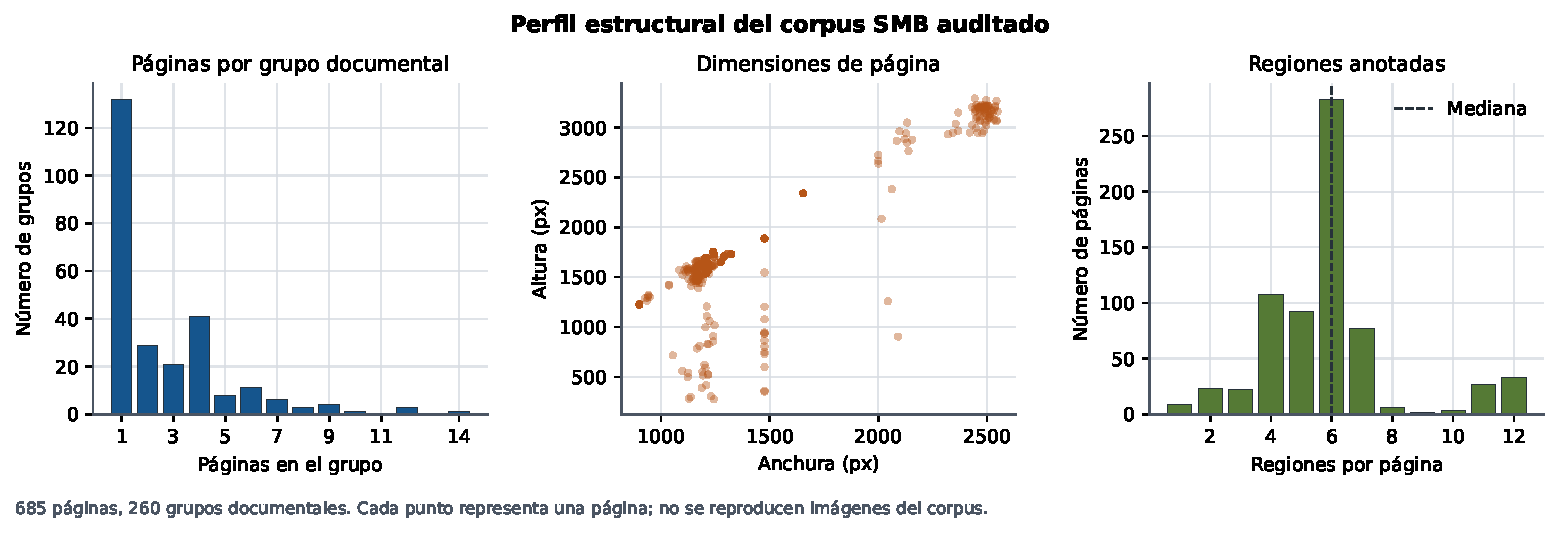
\includegraphics[width=\textwidth]{figures/context/smb-dataset-profile.pdf}
  \caption{Perfil de páginas por grupo documental, dimensiones y regiones anotadas en el inventario completo.
  Fuente: elaboración propia a partir de 685 registros del manifiesto SMB.}
  \label{fig:smb-profile}
\end{figure}

El recorrido desde el conjunto hasta la muestra final se resume en la
Figura~\ref{fig:sample-flow}. No partió exclusivamente de las 618 páginas con anotaciones
válidas, ya que la reconstrucción de página completa no utiliza esos campos. Tras excluir los 53
grupos del piloto v1 y las páginas con relaciones duplicadas o pendientes, quedaron 427 candidatas
de 207 grupos documentales. El recorrido determinista examinó 140 páginas hasta reunir 64 grupos documentales: el estimador
descartó 76 por no poder establecer una escala válida, 75 de ellas pertenecientes al grupo de 618
y una al grupo de 67. Las 64 aceptadas comprenden 56 páginas del primer grupo y ocho del segundo;
estas ocho conservaban píxeles y geometría aptos para la evaluación, aunque les faltara algún texto
regional no usado por los modelos ni por las métricas. La selección de una página por grupo evita
repetir un identificador y facilita la comparación, pero introduce un sesgo de mensurabilidad que debe acompañar
a cualquier conclusión.

\begin{figure}[htbp]
  \centering
  \begin{tikzpicture}[
      node distance=6mm,
      box/.style={draw, rounded corners=2pt, align=center, minimum width=0.82\textwidth,
        minimum height=8mm, fill=blue!5},
      arrow/.style={-{Latex[length=2mm]}, thick}]
    \node[box] (all) {685 páginas procesadas en 260 grupos documentales\\
      618 con anotación válida y 67 con anotación no válida};
    \node[box, below=of all] (candidates) {427 páginas candidatas de 207 grupos documentales\\
      tras excluir grupos v1 y relaciones duplicadas o pendientes};
    \node[box, below=of candidates] (scale) {140 páginas examinadas hasta el cierre\\
      76 rechazadas por escala: 75 del grupo de 618 y una del de 67};
    \node[box, below=of scale, fill=green!8] (sample) {64 páginas de 64 grupos documentales\\
      56 del grupo de 618 y ocho del de 67};
    \draw[arrow] (all) -- (candidates);
    \draw[arrow] (candidates) -- (scale);
    \draw[arrow] (scale) -- (sample);
  \end{tikzpicture}
  \caption{Flujo de selección del inventario a la muestra confirmatoria. Fuente: elaboración
  propia a partir del manifiesto y de la selección congelada.}
  \label{fig:sample-flow}
\end{figure}

\section{Particiones y prevención de fugas}
\label{sec:smb-grouping}
SMB solo publica una partición oficial denominada \texttt{test}; las etiquetas de entrenamiento,
validación y prueba utilizadas en este TFG son, por tanto, roles internos y no nuevas particiones
oficiales. En la comparación principal, los 64 grupos documentales de la muestra v2 se reservaron íntegramente
para inferencia: no se utilizaron para entrenamiento, validación, ajuste de hiperparámetros,
elección de métodos o puntos de control.

La unidad operativa fue el grupo documental identificado por \texttt{source\_group\_id},
obtenido de \texttt{original\_score} al retirar únicamente el sufijo de página \texttt{\_pN}.
Un grupo puede corresponder a un documento, un movimiento o una sección, y no equivale
necesariamente a una composición completa. Las páginas se evaluaron de forma emparejada y las
regiones o recortes se trataron como observaciones anidadas. El manifiesto reconcilió los índices
esperados y comprobó la separación de páginas e identificadores entre roles; en la muestra
principal se retuvo una página por grupo. Esta comprobación no acredita la independencia musical
entre todos los grupos.

Por ejemplo, \texttt{beethoven\_sonata01\_2} aparece en entrenamiento (índices 339--341) y
\texttt{beethoven\_sonata01\_4} en prueba (390--396, con representante 391);
\texttt{mozart\_sonata15\_1} aparece en entrenamiento (652--654) y
\texttt{mozart\_sonata15\_3} en prueba (578). Son movimientos de las mismas sonatas
distribuidos entre roles distintos. No se constató reutilización de las mismas páginas o píxeles,
pero persiste dependencia potencial entre movimientos, secciones o ediciones. Por ello, los
resultados SMB describen documentos retenidos y no certifican generalización a composiciones
completas nunca vistas. No se realizó un análisis de sensibilidad por composición completa;
los manifiestos y resultados congelados se conservan sin redefinir retrospectivamente sus grupos.

El estudio secundario de adaptación se definió después de cerrar aquella comparación, pero antes
de entrenar o consultar sus resultados. Excluyó los 64 grupos documentales v2; asignó al entrenamiento 45 grupos documentales
del piloto v1, con 212 páginas elegibles; y seleccionó entre grupos no utilizados 13 para validación y 20
para prueba, con 35 y 55 páginas elegibles. La selección de punto de control empleó 13 casos fijos
de validación, mientras que la prueba utilizó una página representativa por cada uno de sus 20
grupos. Ningún identificador de grupo cruzó roles y los identificadores de validación y prueba no
habían aparecido en v1 ni v2. Esta separación permite estudiar adaptación dentro del corpus con
documentos distintos de la comparación principal, con la dependencia residual indicada; no
demuestra independencia por composición ni transferencia a otra colección.
La Tabla~\ref{tab:adaptation-split} hace explícitos los tres roles internos y sus denominadores.

\begin{table}[htbp]
  \centering
  \small
  \caption{Roles internos del estudio secundario de adaptación EDSR. No son particiones oficiales
  de SMB. Fuente: elaboración propia a partir del manifiesto congelado.}
  \label{tab:adaptation-split}
  \begin{tabular}{lrrp{0.39\textwidth}}
    \toprule
    Rol & Grupos & Páginas elegibles & Uso \\
    \midrule
    Entrenamiento & 45 & 212 & Muestreo equilibrado de recortes; grupos del piloto v1 \\
    Validación & 13 & 35 & Selección de punto de control sin consultar prueba \\
    Prueba & 20 & 55 & Una página fija por grupo y seis condiciones \\
    \bottomrule
  \end{tabular}
\end{table}

\section{Corpus externo para la prueba profesional}
La prueba de transferencia empleó páginas aportadas por el archivo musical de la Societat Joventut
Musical d'Albal (SJMA), ajenas a SMB. La entidad autorizó el acceso, el procesamiento y la
reproducción de una selección en este trabajo; el estudiante compiló el corpus, pero no se atribuye
la titularidad de las obras, arreglos o ediciones subyacentes. Las páginas HR, LR y reconstruidas
permanecen fuera de Git y no se distribuyen como colección. La memoria reproduce las doce
comparaciones cualitativas predeclaradas, atribuidas y comentadas, para hacer auditables todos los
veredictos y no solo los resultados favorables. Esta autorización acotada no se presenta como permiso
general de publicación o explotación de las partituras.

Se recibieron dieciséis partes de banda de una página. Antes de generar resultados, tres se
asignaron exclusivamente a ingeniería del estimador de pentagrama y una quedó como reserva por
redundancia de sus características de entrada. Las doce restantes, una por obra independiente, se
congelaron como prueba externa. La selección utilizó únicamente tipo de fuente, orientación,
instrumento, densidad, estado documental, presencia de texto y escala estimada; no consultó ninguna
salida de superresolución.

\begin{table}[htbp]
  \centering
  \small
  \caption{Composición del corpus externo congelado. Fuente: elaboración propia a partir del
  manifiesto privado de la SJMA.}
  \label{tab:external-corpus}
  \begin{tabular}{lp{0.27\textwidth}p{0.43\textwidth}}
    \toprule
    Rol & Cantidad & Cobertura de entrada \\
    \midrule
    Ingeniería & 3 obras & Casos usados para corregir el estimador; excluidos de resultados \\
    Prueba & 12 obras & 10 fuentes digitales y 2 escaneos; 8 verticales y 4 horizontales \\
    Reserva & 1 obra & Excluida por redundancia antes de observar salidas \\
    \bottomrule
  \end{tabular}
\end{table}

Entre las doce obras de prueba había siete páginas de notación densa, tres media y dos dispersa;
todas contenían texto. La separación estimada entre líneas de pentagrama abarcó de 10 a 15 píxeles
HR, con mediana 12,75. Las dimensiones variaron entre 1.818 y 2.572 píxeles de anchura y entre 1.818
y 2.629 de altura. Estas propiedades amplían la variedad documental respecto de SMB, pero doce
partes de banda no representan todas las colecciones profesionales.
La composición y las exclusiones previas del corpus se sintetizan en la
Tabla~\ref{tab:external-corpus}.

\section{Degradación controlada}
La evaluación final utilizó el protocolo \texttt{staff-scale-score-v2}. Se mantuvieron seis
condiciones, correspondientes a los factores de ampliación \(\times 2\) y \(\times 4\) y a los
perfiles \emph{clean}, \emph{moderate} y \emph{strong}. En todas ellas la reducción se efectuó con
\texttt{INTER\_AREA}. El perfil limpio no añadió ninguna operación posterior. En el perfil
moderado, el desenfoque gaussiano se definió como
\(\max(0{,}3,0{,}05s)\) píxeles de la imagen de alta resolución, donde \(s\) es la separación
entre líneas de pentagrama; tras la reducción se añadió ruido gaussiano acromático con
\(\sigma=1{,}5\) y compresión JPEG de calidad 80 sin submuestreo de crominancia. En el perfil
fuerte se emplearon \(\max(0{,}3,0{,}15s)\), \(\sigma=2{,}5\) y calidad JPEG 45,
respectivamente. La semilla maestra fue 20260830 y cada aplicación conservó sus parámetros y su
semilla efectiva.
La Tabla~\ref{tab:degradation-v2} permite reproducir los operadores y distingue el perfil limpio de
los dos niveles que añaden desenfoque, ruido y compresión.

\begin{table}[htbp]
  \centering
  \small
  \caption{Operadores del protocolo de degradación final. \(s\) es la separación entre líneas de
  pentagrama medida en la imagen HR. Fuente: elaboración propia.}
  \label{tab:degradation-v2}
  \begin{tabular}{lccc}
    \toprule
    Perfil & Desenfoque gaussiano HR & Ruido tras reducción & JPEG 4:4:4 \\
    \midrule
    Limpio & ninguno & ninguno & ninguno \\
    Moderado & \(\max(0{,}3;0{,}05s)\) & gaussiano acromático, \(\sigma=1{,}5\) & calidad 80 \\
    Fuerte & \(\max(0{,}3;0{,}15s)\) & gaussiano acromático, \(\sigma=2{,}5\) & calidad 45 \\
    \bottomrule
  \end{tabular}
\end{table}

La Figura~\ref{fig:degradation-profiles} traduce estos parámetros a su efecto visual. Se aplica la
misma escala \(\times 4\) y el mismo recorte HR en los tres perfiles: así, las diferencias no se
deben a la obra ni al contenido elegido. La entrada limpia pierde resolución por el submuestreo;
la moderada añade una pérdida visible pero conserva las estructuras principales; y la fuerte hace
más inciertas las alteraciones, separaciones internas y líneas finas. Las LR se amplían por vecino
más próximo solo para compararlas al mismo tamaño, no como método de reconstrucción.

\begin{figure}[htbp]
  \centering
  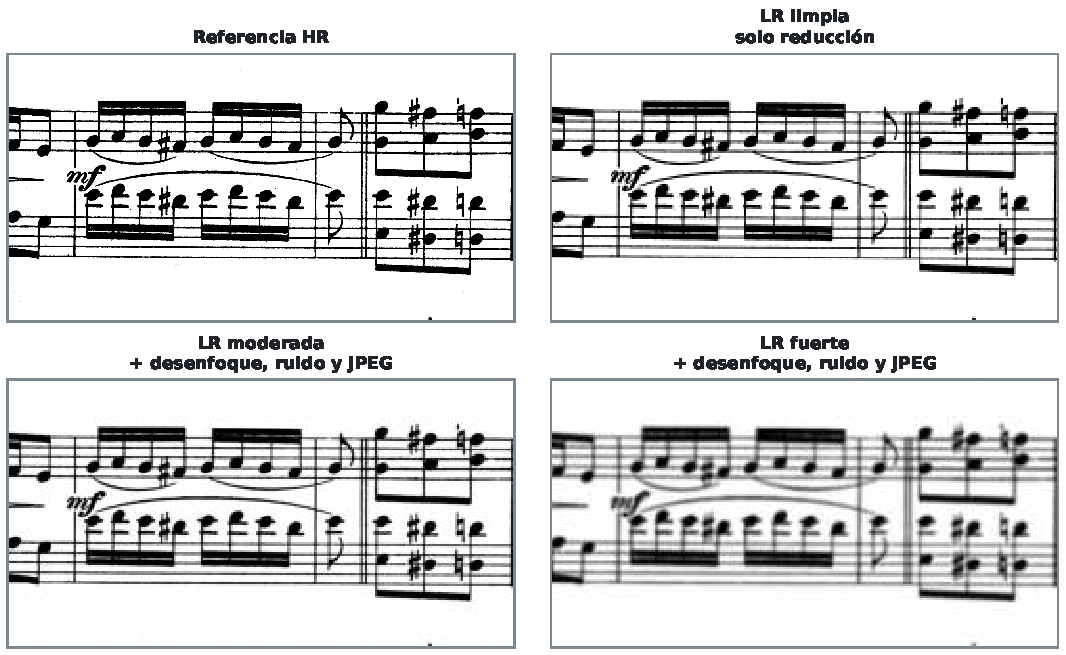
\includegraphics[width=\textwidth]{figures/context/degradation-profiles-x4.pdf}
  \caption[Ejemplo visual de los tres perfiles de degradación]{Efecto de los perfiles limpio,
  moderado y fuerte a escala \(\times 4\) sobre el mismo fragmento. La versión moderada regenerada
  coincide píxel a píxel con la entrada conservada del experimento. Fragmento de
  \emph{Scott Joplin's New Rag}, de Scott Joplin, identificado como
  \texttt{joplin\_newrag}. Fuente: elaboración propia con el protocolo v2 a partir de SMB
  \cite{smbDatasetCard}.}
  \label{fig:degradation-profiles}
\end{figure}

La normalización por escala de pentagrama fue una corrección metodológica necesaria. Una primera
ejecución completa, conservada solo como piloto de desarrollo y prueba de estrés, había utilizado
desenfoques expresados en píxeles absolutos que se calibraron sobre fragmentos sintéticos con
pentagramas mayores. Al transferirlos a páginas SMB de escalas variables, algunas condiciones
moderadas y fuertes dejaron de representar la severidad prevista. Antes de inspeccionar resultados
del nuevo protocolo se congeló una muestra nueva de 64 páginas pertenecientes a 64 grupos documentales, sin
páginas ni identificadores del piloto. La separación de pentagrama de estas páginas abarca de 6,526 a 18,275
píxeles, con mediana 9,996. Por tanto, los resultados finales se refieren solo a páginas SMB para
las que el estimador determinista pudo medir esta escala, no a todo SMB ni a escaneos reales no
controlados.

La Figura~\ref{fig:staff-scale} muestra la cobertura. La mayoría de grupos se concentra entre 8 y
11 píxeles, con un segundo grupo pequeño entre 16 y 18 píxeles. La fórmula hace que el desenfoque
crezca con la estructura observada: dentro de la muestra, \(\sigma\) abarca aproximadamente
0,33--0,91 píxeles HR en el perfil moderado y 0,98--2,74 en el fuerte. De este modo, una misma
etiqueta de severidad conserva una relación comparable con el pentagrama, aunque no convierte las
degradaciones sintéticas en una simulación de todos los escaneos reales.

\begin{figure}[htbp]
  \centering
  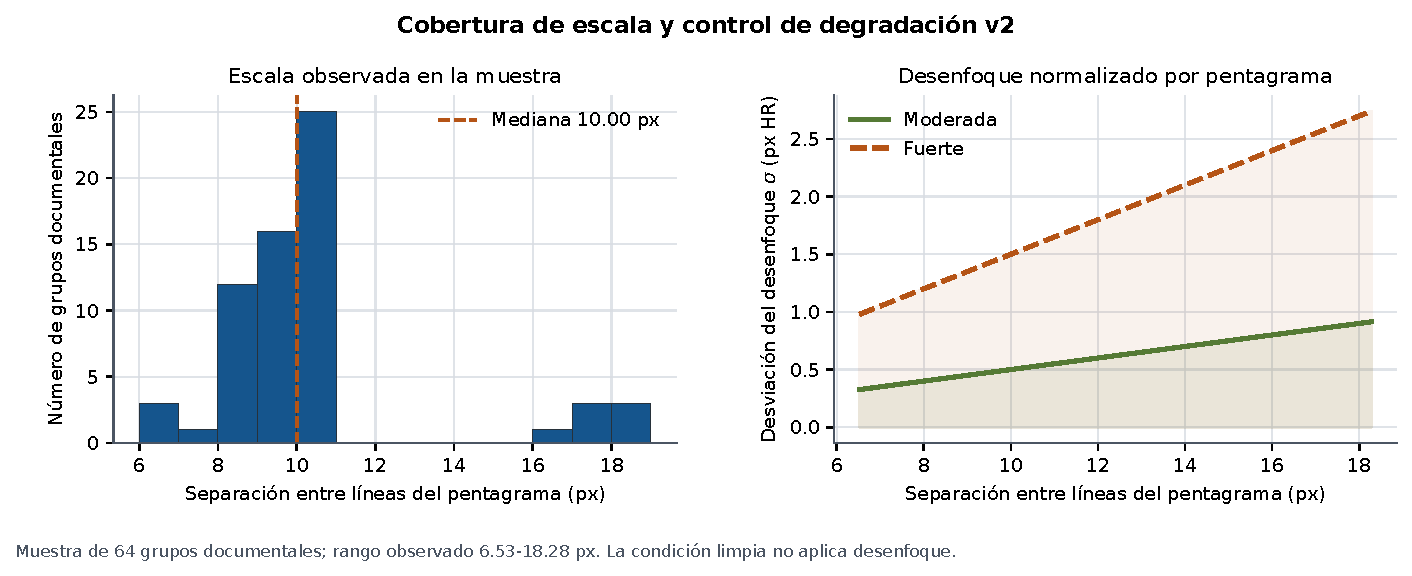
\includegraphics[width=\textwidth]{figures/context/staff-scale-and-blur.pdf}
  \caption[Escala de pentagrama y desenfoque en la muestra v2]{Distribución de separación entre líneas y desenfoque resultante en la muestra v2.
  Fuente: elaboración propia a partir de los 64 grupos documentales seleccionados y del protocolo congelado.}
  \label{fig:staff-scale}
\end{figure}
